At the backbone of all classical protocols described in Section \ref{section:protocols}, it lies the need to generate random uniform distributions of either qubit states, Bloch vectors or shared randomness in $\mathbb{R^3}$. In Figure \ref{fig:results_random_states}, we can see that applying random unitary transformations to zero qubit states leads to uniformly distributed random qubit pure states, which can later be transformed into random Bloch vectors or normalized random vectors in $\mathbb{R^3}$ as needed. These random states are also the seed to compute random POVMs with rank-1 projectors, as described in Section \ref{section:povm_generation}. Hence, once proven we have means to generate random states and rank-1 POVMs, we can address the measurement process. 
\begin{figure}[h]
\centering
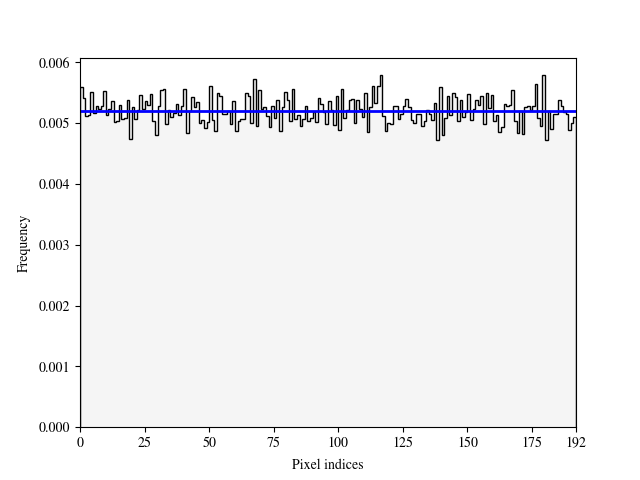
\includegraphics[width=\textwidth]{images/random_bloch_healpix.png}
\caption{In this histogram we see how the frequency distribution of $N=10^4$ random qubit states generated with \cite{software2023} follows a random uniform distribution of state vectors along the Bloch sphere (blue solid line). The frequencies are binned by HEALPix indices corresponding to an equal-area iso-latitude partition of the Bloch sphere with resolution $\mathit{NSIDE}=4$.}
\label{fig:results_random_states}
\end{figure}

The outcome probabilities for a given random POVM measure can be obtained analytically using the Born's rule, but we have gone a step further and used simulators and noisy intermediate-scale quantum computers (see Table \ref{table:quantum_resources}) to calculate such probabilities and compare them to the theoretical ones as described in \ref{section:quantum_circuit}. 
\newline
\begin{table}[h!]
\centering
\begin{tabular}{c c c c c} 
 \toprule
 Name & Qubits & Quantum Volume & CNOT Error & Readout Error \\ [1ex] 
 \midrule
 Nairobi & 7 & 32 & 0.01357 & 0.0227 \\ 
 Perth & 7 & 32 & 0.01733 & 0.0188 \\
 Oslo & 7 & 32 & 0.01 & 0.01667 \\
 Jakarta & 7 & 16 & 0.00773 & 0.0258 \\
 Lagos & 7 & 32 & 0.007243 & 0.0145 \\ 
 \bottomrule
\end{tabular}
\caption{Properties of Noisy Intermediate-Scale Quantum computers available at \href{https://quantum-computing.ibm.com}{IBM Quantum} to compute the prepare-and-measure outcome probabilities.}
\label{table:quantum_resources}
\end{table}

A summary of the achievable performances for a particular state and POVM measure can be found in Table \ref{table:quantum_results}. Quantum computers currently available to the public are limited to running circuits with a maximum of twenty thousand shots. This results in less accuracy compared to the Qiskit Aer simulator, which can perform simulations with a full range of shots, as we will see later in the classical simulation results discussion. A comprehensive benchmark of IBM's free-access simulators and quantum computers for the same prepare-and-measure scenario can be found in Appendix \ref{section:benchmark}.

%\textit{Convergence plots, classical vs. quantum vs. theoretical probabilities}
%\textit{Kullback-Leibler divergence plots}
%\textit{Bell scenario joint probabilities convergence}
%\textit{CHSH inequality}

\afterpage{%
    \clearpage
    \thispagestyle{empty}
    \begin{landscape}
        \centering 
        \begin{tabular}{llll}
            A & B & C & D \\
        \end{tabular}
        \captionof{table}{Example of probability distributions obtained with different IBM Quantum systems and simulators for a prepare-and-measure scenario with state $\ket{\Psi}=\frac{3 + i \sqrt{3}}{4} \ket{0} - \frac{1}{2} \ket{1}$ and POVM measure $\mathbb{P}_4 = \{\frac{1}{2}\ket{0}\bra{0}, \frac{1}{2}\ket{1}\bra{1}, \frac{1}{2}\ket{+}\bra{+}, \frac{1}{2}\ket{-}\bra{-} \}$}
        \label{table:quantum_results}
    \end{landscape}
    \clearpage% Flush page
}